\documentclass[a4paper,14pt]{extarticle}
\usepackage[utf8]{inputenc}
\usepackage[russian]{babel}
\usepackage{graphicx}
\usepackage[top=0.8in, bottom=0.8in, left=0.8in, right=0.8in]{geometry}
\usepackage{pgfplots}
\usepackage{amsmath}
\usepackage{setspace}
\usepackage{titlesec}
\usepackage{float}
\usepackage{chngcntr}
\usepackage{pgfplots}
\usepackage{amsfonts}
\usepackage{pgfplotstable}
\usepackage{multirow}
\usepackage{karnaugh-map}
\usepackage{tikz,xcolor}
\usepackage{listings}

\titleformat{\section}[hang]
  {\bfseries}
  {}
  {0em}
  {\hspace{-0.4pt}\large \thesection\hspace{0.6em}}
  
  
\titleformat{\subsection}[hang]
  {\bfseries}
  {}
  {0em}
  {\hspace{-0.4pt}\large \thesubsection\hspace{0.6em}}

\newcommand{\nx}{\overline{x}}
\newcommand{\p}{0.31}
\newcommand{\scale}{1.4}

\counterwithin{figure}{section}
\counterwithin{equation}{section}
\counterwithin{table}{section}

\lstdefinestyle{CStyle}{
    basicstyle=\footnotesize,
    breakatwhitespace=false,         
    breaklines=true,                 
    captionpos=b,                    
    keepspaces=true,                 
    numbers=left,                    
    numbersep=5pt,                  
    showspaces=false,                
    showstringspaces=false,
    showtabs=false,                  
    tabsize=2,
    language=C
}

\begin{document}
\begin{titlepage}
\centering
\small Балтийский государственный технический университет «Военмех» им. Д.Ф.Устинова \\
\vspace{3cm}
\normalsize Кафедра И5\\
«Информационные системы и программная инженерия»\\
\vspace{3cm}
\textbf{Практическое задание №6}\\
по дисциплине Основы программирования на тему\\ 
\textbf{«Строки»}\\
\vfill

\begin{flushleft}
\textbf{Выполнил:}
\hfill {Мальцев А.С.} \\
\hfill {Группа И595} \\
\vspace{1cm}
\textbf{Преподаватель:}
\hfill {Лазарева Т.И.} \\
\end{flushleft}
\vspace{3cm}

{\centering Санкт-Петербург \\
\vspace{0.15cm}
2019}
\end{titlepage}
\setcounter{page}{2}
\section{Цель работы}
Ознакомиться с организацией строк в языке Си, изучить библиотечные функции обработки строк и символов.

\section{Ход работы}
\subsection{Задание 1}
Дана строка символов до точки. Определить, сколько слов, состоящих из пяти и более символов, содержит данная строка.\\
\textit{Исходные данные:} строка символов до точки.\\
\textit{Результирующие данные:} значение счетчика слов, длинной более 4 символов.\\
\begin{center}
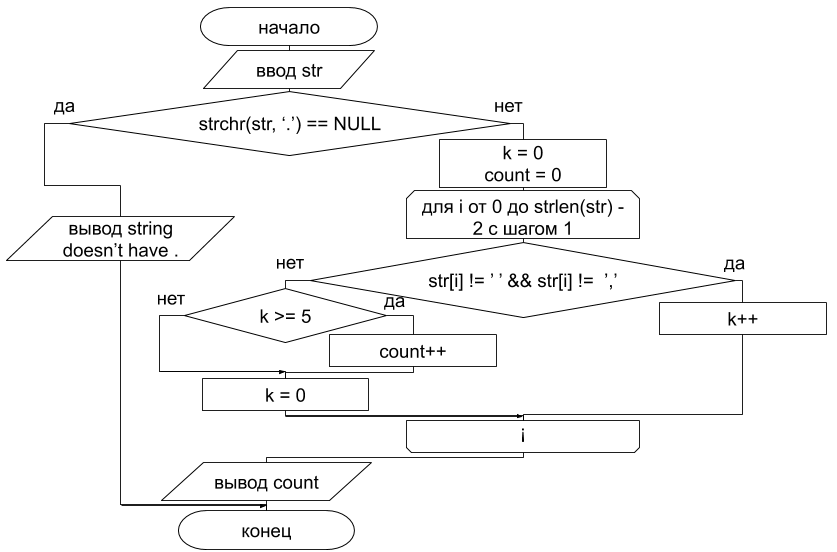
\includegraphics[scale=0.6]{lab6-1.png}\\
Схема программы
\end{center}
\lstinputlisting[language=c, frame=single, style=CStyle]{../1.c}
\begin{center}
Текст программы\\
\vspace{0.6cm}
\begin{tabular}{|l|l|}
\hline
\multicolumn{1}{|c|}{Исходные данные}& \multicolumn{1}{|c|}{Вывод программы}\\
\hline
hello world, my name is Alex. & 2 \\
\hline
hi mate & string doesn't have . \\
\hline
what is going on here. & 1 \\
\hline
\end{tabular}\\
\vspace{0.3cm}
Результаты тестирования
\end{center}

\subsection{Задание 2}
Строка содержит запись арифметического выражения на языке Си. В выражении могут использоваться операции «+», «-», «*», «\%», функции sin(), cos(), tan(). Получить строку, содержащую запись этого выражения на языке Паскаль. (Константы, идентификаторы, операции «+», «-», «*» и функции sin() и cos() на Паскале записываются так же, как на Си, операцию «\%» следует заменить на « mod », функции вычисления тангенса в Паскале не существует, нужно использовать отношение синуса к косинусу.)\\
\textit{Исходные данные:} строка-выражение на Си.\\
\textit{Результирующие данные:} строка-выражение на Паскале.\\
\begin{center}
% 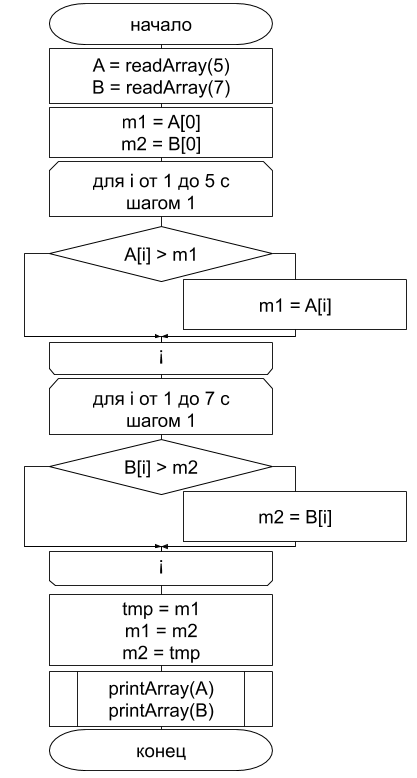
\includegraphics[scale=0.6]{lab5-1.png}\\
Схема программы
\end{center}
\lstinputlisting[language=c, frame=single, style=CStyle]{../2.c}
\begin{center}
Текст программы\\
\vspace{0.6cm}
\begin{tabular}{|l|l|}
\hline
\multicolumn{1}{|c|}{Исходные данные}& \multicolumn{1}{|c|}{Вывод программы}\\
\hline
1 - tan(9 * tan(4)) & 1 - sin(9 * sin(4) / cos(4)) / cos(9 * sin(4) / cos(4)) \\
\hline
tan(4 \% 2) & sin(4 mod 2) / cos(4 mod 2) \\
\hline
\end{tabular}\\
\vspace{0.3cm}
Результаты тестирования
\end{center}
\end{document}
